% \begin{frame}[squeeze]{Analiza}
\begin{frame}{Minimax}

  \textbf{Minimax} jest algorytmem przeszukiwania przestrzeni stanów rozgrywki dla gier dwuosobowych.
  
  \ldots

  % \begin{itemize}
  %   \myitem Wouter van Oortmerssen, 1993
  %   \myitem Powstał w dwóch celach:
  %   \begin{itemize}
  %     \item Jak najmniejszy kompilator (1024B);
  %     \item Jak najbardziej zaciemniona składnia.
  %   \end{itemize}
  %   \myitem Używa zmiennych, arytmetyki stosowej, wyrażeń lambda itd.
  % \end{itemize}

  % \begin{figure}
  %   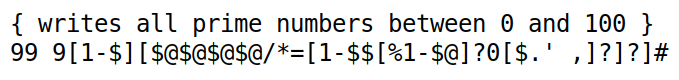
\includegraphics[width=10cm]{figures/false.png}
  % \end{figure}

	% \begin{itemize}
	% \item[$d(u,v)$] --  długość ścieżki z $u$ do $v$
	% \item[$\SPHERE{v}{r}$] $= \{u: d(u,v) = r\}$
	% \item[$\DISC{v}{r}$] $ = \{u: d(u,v)\leq r\}$
	% \end{itemize}

	%  \begin{tikzpicture}[remember picture, overlay]
 	
         \node [shift={(9cm,-3.4cm)}]  at (current page.north west)
            {
            \tikzstyle{place}=[circle,draw=black!100,fill=blue,thin, inner sep=0pt,minimum size=2mm]
            \tikzstyle{red place}=[circle,draw=black!100,fill=yellow!100,thin, inner sep=0pt,minimum size=2mm]

            \begin{tikzpicture}


                \node at (-1,0) [red place]  (1) {};
                \node at (-0.6,0.8) [red place]  (2) {};
                \node at ( -0.1,0.6) [red place]  (3) {};
                \node at ( -0.4,-0.5) [red place]  (4) {};
                \node at ( 0,0) [ red place]  (5) {v};
                \node at (0.75,-0.75) [red place]  (6) {};
                \node at ( 1,0.3) [red place] (7) {};
                \node at (1.5,-0.35) [red place]  (8) {};
                \node at (0.1,-0.85) [red place]  (9) {};


                \node at ( -1.5,-0.3) [place]  (10) {};
                \node at ( -1.5,0.5) [place]  (11) {};
                \node at ( -1.2,1) [place]  (12) {};
                \node at ( -0.2,1.2) [place]  (13) {};
                \node at ( 0.8,0.8) [place]  (14) {};
                \node at ( 1.6,0.6) [place]  (15) {};
                \node at ( 1.9,-0.8) [place]  (16) {};
                \node at ( 1.9,0) [place]  (17) {};
                \node at ( -0.3,-1.2) [place]  (18) {};
                \node at ( 0.5,-1.3) [place]  (19) {};


                \draw [->] (1) to (2);
                \draw [->] (2) to (3);
                \draw [<-] (3) to (7);
                \draw [->] (3) to (5);
                \draw [<-] (5) to (6);
                \draw [<-] (6) to (8);
                \draw [->] (8) to (7);
                \draw [<-] (5) to (4);
                \draw [->] (1) to (4);
                \draw [<-] (6) to (9);
                \draw [<-] (4) to (9);

                \draw [<-] (1) to (10);
                \draw [<-] (1) to (11);
                \draw [<-] (2) to (12);
                \draw [<-] (2) to (13);
                \draw [<-] (7) to (14);
                \draw [<-] (7) to (15);
                \draw [<-] (8) to (16);
                \draw [<-] (8) to (17);
                \draw [<-] (9) to (18);
                \draw [<-] (9) to (19);


          
            \end{tikzpicture}

            };
        
\end{tikzpicture}

	% \vspace{2cm}	

  %   \begin{twierdzenie}[Propagacja minimum]
  %   	Niech $M_{v,r}$  oznacza zdarzenie, że $v$ nadaje w rundzie $r$ oraz
  %       niech $\mathcal{G} =(V,E)$ będzie graf skierowanym i niech $v\in V$.
  %       Załóżmy, że $\SPHERE{v}{r}\neq \emptyset$.
  %       Wówczas zdarzenia $M_{v,0}, \ldots M_{v,r}$ \underline{są niezależne}
  %       oraz
  %       $$
  %         \Pr[M_{v,j}] = |\SPHERE{v}{j}|\Big/{|\DISC{v}{j}|}~.
  %       $$
  %   \end{twierdzenie}

\end{frame}
